%
% beschreibung.tex -- Beschreibung von Graphen mit Matrizen
%
% (c) 2020 Prof Dr Andreas Müller, Hochschule Rapperswil
%
\section{Beschreibung von Graphen mit Matrizen
\label{buch:section:beschreibung-von-graphen-mit-matrizen}}
\rhead{Beschreibung mit Matrizen}
Ein Graph ist eine Menge von Knoten, die untereinander mit Kanten
verbunden sind.
Graphen können zum Beispiel verwendet werden um Netzwerke zu beschreiben,
aber auch viele andere Datenstrukturen.
Die Knoten können einzelne Objekte beschreiben, die Kanten beschreiben
dann Beziehungen zwischen diesen Objekten.

\subsection{Definition von Graphen
\label{subsection:definition-von-graphen}}
In der Einleitung zu diesem Abschnitt wurde bereits eine informelle
Beschreibung des Konzeptes eines Graphen gegeben.
Um zu einer Beschreibung mit Hilfe von Matrizen kommen können,
wird eine exakte Definition benötigt.
Dabei werden sich einige Feinheiten zeigen, die für Anwendungen wichtig
sind und sich in Unterschieden in der Definition der zugehörigen Matrix 
äussern.

\subsubsection{Ungerichtete Graphen}
Die Grundlage für alle Arten von Graphen ist eine Menge $V$ von {\em Knoten},
auch {\em Vertices} genannt.
\index{Knoten}%
\index{Vertex}%
Die Unterschiede zeigen sich in der Art und Weise, wie die Knoten
mit sogenannten die Kanten 
\index{Kante}%
verbunden werden.
Bei einen ungerichteten Graphen sind die beiden Endpunkte einer Kante
gleichwertig, es gibt keine bevorzugte Reihenfolge oder Richtung der
Kante.
Eine Kante wird daher vollständig spezifiziert, wenn wir die
Menge der Endpunkte kennen.
Dies führt auf die folgende Definition eines ungerichteten Graphen.

\begin{definition}
\label{buch:def:ungerichteter-graph}
\index{Graph!ungerichteter}%
\index{ungerichteter Graph}%
Ein {\em ungerichteter Graph} ist eine endliche Menge $V$ von {\em Knoten}
und eine Menge $E$ von zweielementigen Teilmengen 
\[
E \subset \{\, \{a,b\}\subset V\,|\, a\ne b\}.
\]
Die Elemente von $E$ heissen {\em Kanten} ({\em edges}).
\end{definition}

Man beachte, dass es keine Kante gibt, die einen Knoten $a\in V$
mit sich selbst verbindet, da die zugehörige Menge $\{a,a\}=\{a\}$
nicht aus zwei verschiedenen Elementen besteht, wie die
Definition~\ref{buch:def:ungerichteter-graph} dies verlangt.

Ein elektrisches Netzwerk von ohmschen Widerständen kann mit Hilfe
eines ungerichteten Graphen beschrieben werden.
Ohmsche Widerstände hängen nicht von der Richtung des Stromflusses
durch die Widerstände ab.
Will man Spannungen und Ströme in einem solchen Netzwerk berechnen,
ist auch das Fehlen von Schleifen, die von $a$ zu $a$ führen, kein
Verlust.
Die Endpunkte solcher Widerstände wären immer auf gleichem Potential,
es würde daher kein Strom fliessen, sie haben daher keinen Einfluss auf
das Verhalten des Netzwerkes und können weggelassen werden.

\subsubsection{Gerichtete Graphen}
In vielen Anwendungen sind die Endpunkte einer Kante nicht austauschbar.
In einem Strassennetz sind Einbahnstrassen nicht in beiden Richtungen
befahrbar.
Anfangs- und Endpunkt einer Kante müssen in einem solche Graphen
unterschieden werden.
Eine zweielementige Menge ist daher nicht mehr eine geeignete Abstraktion
für die Kante, ein (geordnetes) Paar von Vertizes passt besser.

\begin{definition}
\label{buch:def:gerichteter-graph}
\index{Graph!gerichteter}%
\index{gerichteter Graph}%
Ein {\em gerichteter Graph} ist eine endliche Menge $V$ von Knoten
und eine Menge $E \subset V\times V$ von gerichteten Kanten.
Ausserdem gibt es zwei Abbildungen
\[
\begin{aligned}
a&\colon E\to V: (p,q) \mapsto a((p,q)) = p
\\
e&\colon E\to V: (p,q) \mapsto e((p,q)) = q.
\end{aligned}
\]
Der Knoten $a(k)$ heisst der {\em Anfangspunkt} der Kante $k\in E$,
$e(k)$ heisst der {\em Endpunkt}.
\end{definition}

In einem gerichteten Graphen gehört also zu jeder Kante auch eine Richtung
und die Unterscheidung von Anfangs- und Endpunkt einer Kante ist sinnvoll
geworden.
Ausderdem ist eine Kante $(a,a)$ wohldefiniert, also eine Kante, die vom
Knoten $a$ wieder zu $a$ zurückführen.

Man kann einen ungerichteten Graphen in einen gerichteten Graphen
verwandeln, indem wir jede Kante $\{a,b\}$ durch zwei Kanten 
$(a,b)$ und $(b,a)$ ersetzen.
Aus dem ungerichteten Graphen $(V,E)$ mit Knotenmenge $V$ und Kantenmenge
$E$ wird so der gerichtete Graph
$(V,E')$ mit der Kantenmenge
\begin{equation*}
E' 
=
\{
(a,e)
\,|\,
\{a,e\}\in E
\}.
\end{equation*}
Eine umgekehrte Zuordnung eines ungerichteten Graphen zu einem gerichteten
Graphen ist nicht möglich, da eine ``Schleife'' $(a,a)$ nicht in Kante
des ungerichteten Graphen abgebildet werden kann.

In einem gerichteten Graphen kann man sinnvoll von gerichteten Pfad
sprechen.
\index{Pfad}%
Ein {\em Pfad} $\gamma$ in einem gerichteten Graphen $(V,E)$ ist eine Folge
$k_1,\dots,k_r\in E$ von Kanten derart, dass $e(k_i) = a(k_{i+1})$
für $i=1,\dots,r-1$.
Dies bedeutet, dass der Endpunkt jeder Kante mit dem Anfangspunkt der
nachfolgenden Kante übereinstimmt.
Die {\em Länge} des Pfades $\gamma=(k_1,\dots,k_r)$ ist $|\gamma|=r$.

Eine naheliegende Beschreibung eines gerichteten Graphen mit Hilfe einer
Matrix kann man wie folgt erhalten.
Zunächst werden die Knoten aus der Menge $V$ durch die Zahlen
$1,\dots,n$ mit $n=|V|$ ersetzt.
Diese Zahlen werden dann als Zeilen- uns Spaltenindizes interpretiert.
Die zum Graphen gehörige Matrix enthält die Einträge
\begin{equation}
g_{ij}
=
\begin{cases}
1&\qquad  (j,i) \in E\\
0&\qquad  \text{sonst.}
\end{cases}
\label{buch:graphen:eqn:linkmatrix}
\end{equation}
Die Matrix $G$ hat also genau dann einen nicht verschwindenden
Matrixeintrag in Zeile $i$ und Spalte $j$, wenn es eine Verbindung
von Knoten $j$ zu Knoten $i$ gibt.
% XXX Abbildung Graph und Verbindungs-Matrix
Die Beschreibung des Graphen mit der Matrix $G$ nach
\eqref{buch:graphen:eqn:linkmatrix} ermöglicht bereits, eine interessante
Aufgabe zu lösen.

\begin{satz}
\label{buch:graphen:pfade-der-laenge-n}
Der gerichtete Graph $([n],E)$ werde beschrieben durch die Matrix $G$.
Dann gibt das Element in Zeile $j$ und Spalte $i$ von $G^n$ die Anzahl
der Wege der Länge $n$ an, die von Knoten $i$ zu Knoten $j$ führen.
Insbesondere kann man die Definition~\eqref{buch:graphen:eqn:linkmatrix}
formulieruen als in Zeile $j$ und Spalte $i$ der Matrix steht die Anzahl
der Pfade der Länge $1$, die $i$ mit $j$ verbinden.
\end{satz}

\begin{proof}[Beweis]
Es ist klar, dass $G^1$ die genannte Eigenschaft hat.
Wir beweisen, dass $G^n$ Pfade der Länge $n$ zählt, mit Hilfe von
vollständiger Induktion.
Zur Unterscheidung schreiben wir $G^{(n)}$ für die Matrix, die in Zeile
$j$ und Spalte $i$ die Anzahl der Pfade der Länge $n$ von $i$ nach $j$
enhält.
Die zugehörigen Matrixelemente schreiben wir $g_{ji}^{n}$ bzw.~$g_{ji}^{(n)}$.
Wir haben also zu zeigen, dass $G^n = G^{(n)}$.

Wir nehmen daher an, dass bereits bewiesen ist, dass das Element in Zeile
$j$ und Spalte $i$ von $G^{n-1}$ die Anzahl der Pfade der Länge $n-1$
zählt, dass also $G^{n-1}=G^{(n-1)}$.
Dies ist die Induktionsannahme.

Wir bilden jetzt alle Pfade der Länge $n$ von $i$ nach $k$.
Ein Pfad der Länge besteht aus einem Pfad der Länge $n-1$, der von $i$ zu
einem beliebigen Knoten $j$ führt, gefolgt von einer einzelnen Kante,
die von $j$ nach $k$ führt.
Ob es eine solche Kante gibt, zeigt das Matrixelement $g_{kj}$ an.
Das Element in Zeile $j$ und Spalte $i$ der Matrix $G^{(n-1)}$ gibt
die Anzahl der Wege von $i$ nach $j$ an.
Es gibt also $g_{kj}\cdot g_{ji}^{(n-1)}$ Wege der Länge $n$, die von $i$
nach $k$ führen, aber als zweitletzten Knoten über den Knoten $j$ führen.
Die Gesamtzahl der Wege der Länge $n$ von $i$ nach $k$ ist daher
\[
g_{ki}^{(n)}
=
\sum_{j=1}^n g_{kj} g_{ji}^{(n-1)}.
\]
In Matrixschreibweise bedeutet dies
\[
G^{(n)}
=
G\cdot G^{(n-1)}
=
G\cdot G^{n-1}
=
G^n.
\]
Beim zweiten Gleichheitszeichen haben wir die Induktionsannahme
verwendet.
\end{proof}

Die Definition~\eqref{buch:graphen:eqn:linkmatrix} der Matrix, die den
Graphen beschreibt, lässt sich natürlich auch auf einen ungerichteten
Graphen verallgemeinern.
Die entstehende Matrix hat dann aber die zusätzlichen Eigenschaften, dass
alle Diagonalelemente $0$ sind und dass die Matrix symmetrisch ist.
Auch im Fall eines ungerichteten Graphen kann die Matrix dazu verwendet
werden, die Anzahl der Pfade zu zählen.

Der Satz~\ref{buch:graphen:pfade-der-laenge-n} ermöglicht auch, einen 
Algorithmus für den sogenannten Durchmesser eines Graphen zu formulieren.

\begin{definition}
\index{Durchmesser eines Graphen}%
\index{Graph!Durchmesser des}%
Der {\em Durchmesser} eines Graphen ist die kürzeste Länge $d$ derart, dass
es zwischen zwei beliebigen Knoten einen Pfad der Länge $\le d$ gibt.
\end{definition}

Der Durchmesser $d$ eines Graphen ist der kleinste Exponent derart,
dass $G^d$ keine ausserdiagonalen Einträge $0$ hat.
Die Diagonalelemente von $G^n$ zählen die Anzahl der geschlossenen Pfade
der Länge $n$, die durch einen Knoten führen.
Diese können für den Durchmesser ignoriert werden.
Man kann also Potenzen $G^n$ berechnen bis keine Einträge $0$ mehr vorhanden
sind.

\begin{beispiel}
\begin{figure}
\centering
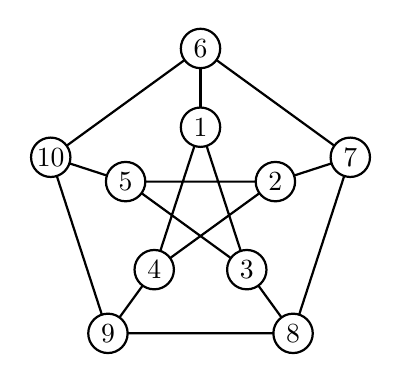
\begin{tikzpicture}[>=latex,thick]
\def\l{0.25}
\def\r{1}
\def\punkt#1{({\r*sin(((#1)-1)*72)},{\r*cos(((#1)-1)*72)})}
\def\R{2}
\def\Punkt#1{({\R*sin(((#1)-6)*72)},{\R*cos(((#1)-6)*72)})}
\draw \Punkt{6} -- \Punkt{7} -- \Punkt{8} -- \Punkt{9} -- \Punkt{10} -- cycle;
\draw \punkt{1} -- \punkt{3} -- \punkt{5} -- \punkt{2} -- \punkt{4} -- cycle;
\foreach \k in {1,...,5}{
	\draw \punkt{\k} -- \Punkt{(\k+5)};
	\fill[color=white] \punkt{\k} circle[radius=\l];
	\node at \punkt{\k} {$\k$};
	\draw \punkt{\k} circle[radius=\l];
}
\foreach \k in {6,...,10}{
	\fill[color=white] \Punkt{\k} circle[radius=\l];
	\node at \Punkt{\k} {$\k$};
	\draw \Punkt{\k} circle[radius=\l];
}
\end{tikzpicture}
\caption{Peterson-Graph mit zehn Knoten.
\label{buch:figure:peterson}}
\end{figure}
Der Peterson-Graph hat die Matrix
\[
G
=
\begin{pmatrix}
%1  2  3  4  5  6  7  8  9 10
 0& 0& 1& 1& 0& 1& 0& 0& 0& 0\\ %  1
 0& 0& 0& 1& 1& 0& 1& 0& 0& 0\\ %  2
 1& 0& 0& 0& 1& 0& 0& 1& 0& 0\\ %  3
 1& 1& 0& 0& 0& 0& 0& 0& 1& 0\\ %  4
 0& 1& 1& 0& 0& 0& 0& 0& 0& 1\\ %  5
 1& 0& 0& 0& 0& 0& 1& 0& 0& 1\\ %  6
 0& 1& 0& 0& 0& 1& 0& 1& 0& 0\\ %  7
 0& 0& 1& 0& 0& 0& 1& 0& 1& 0\\ %  8
 0& 0& 0& 1& 0& 0& 0& 1& 0& 1\\ %  9
 0& 0& 0& 0& 1& 1& 0& 0& 1& 0   % 10
\end{pmatrix}
\]
Durch Nachrechnen kann man bestätigen, dass $G^3$ keine
Ausserdiagonalelemente $0$ enthält:
\[
G^3
=
\begin{pmatrix}
 0& 2& 5& 5& 2& 5& 2& 2& 2& 2\\
 2& 0& 2& 5& 5& 2& 5& 2& 2& 2\\
 5& 2& 0& 2& 5& 2& 2& 5& 2& 2\\
 5& 5& 2& 0& 2& 2& 2& 2& 5& 2\\
 2& 5& 5& 2& 0& 2& 2& 2& 2& 5\\
 5& 2& 2& 2& 2& 0& 5& 2& 2& 5\\
 2& 5& 2& 2& 2& 5& 0& 5& 2& 2\\
 2& 2& 5& 2& 2& 2& 5& 0& 5& 2\\
 2& 2& 2& 5& 2& 2& 2& 5& 0& 5\\
 2& 2& 2& 2& 5& 5& 2& 2& 5& 0
\end{pmatrix}
\]
Daraus kann man jetzt ablesen, dass der Durchmesser des Petersongraphen
$d=5$ ist.
Man kann aber auch mehr ablesen:
\begin{itemize}
\item
Es gibt keine geschlossenen Pfade der Länge $\le 3$.
\item
Zwischen benachbarten Knoten gibt es jeweils $5$ Pfade der Länge $3$,
zwischen nicht benachbarten Knoten gibt es genau $2$ Pfade der Länge $3$.
\qedhere
\end{itemize}
\end{beispiel}

Das Beispiel illustriert, wie sich Zählaufgaben von Pfaden leicht mit dem
Matrizenprodukt erledigen lassen.
Trotzdem ist der Algorithmus nicht unbedingt effizient, da der Aufwand
zur Berechnung des Matrizenproduktes relativ gross sein kann.
Für den Peterson-Graphen können die gefundenen Aussagen über die Anzahl
von Pfaden durch Ausnützung der Symmetrien des Graphen leichter direkt
gefunden werden.

\subsubsection{Beschriftete Graphen}
Bei der Beschreibung eines elektrischen Netzwerkes mit Hilfe eines
ungerichteten Graphen muss jeder Kante zusätzlich ein Widerstandswert
zugeordnet werden.
Dies ist, was eine Beschriftung einer Kante bewerkstelligt.

\begin{definition}
Eine Beschriftung mit Elementen der Menge $L$
eines gerichteten oder ungerichteten Graphen $G=(V,E)$ 
ist eine Abbildung $l\colon E\to L$.
\end{definition}

\subsection{Die Adjazenz-Matrix und Laplace-Matrix
\label{subsection:adjazenz-und-laplace-matrix}}
Die Beschreibung mit der Matrix~\eqref{buch:graphen:eqn:linkmatrix}
``vergisst'' den ``Namen'' der Kante, die eine Verbindung zwischen zwei
Knoten herstellt.
Damit ist sie keine geeignete Grundlage, um beschriftete Graphen einer
Matrixbeschreibung zuzuführen.
Eine solche muss eine Matrix verwenden, nicht nur das Vorhandensein einer
Verbindung wiedergibt, sondern ausdrückt, welche Kante welche beiden
Knoten miteinander verbindet.
Dies führt auf die sogenannte Ajazenz-Matrix.

\begin{definition}
\label{buch:def:adjazenz-matrix}
Ist $G=(V,E)$ ein gerichteter Graph mit $n=|G|$ Vertizes und $m=|E|$ Kanten,
dann ist die zugehörige {\em Adjazenz-Matrix} $A=A(G)$ eine $n\times m$-Matrix.
In der Spalte $k$ wird der Anfangspunkt der Kante $k$ mit $-1$, der Endpunkt
mit $+1$ angezeigt, die übrigen Einträge sind $0$.
$A$ hat also die Matrixelemente
\begin{equation}
a_{ik}
=
\begin{cases}
-1&\qquad $i=a(k)\\
+1&\qquad $i=e(k)\\
0&\qquad\text{sonst}
\end{cases}
\label{buch:eqn:ajazenz-matrix}
\end{equation}
\end{definition}

Der wesentliche Unterschied dieser Definition von der Matrix $H$ 
liegt in der Bedeutung der Einträge.
Für $H$ drückt ein nicht verschwindendes Matrixelement das Vorhandensein
einer Kante aus, in $A$ ist es die Tatsache, dass in diesem Knoten
eine Kante endet.



